\section{Desarrollo} 
\begin{itemize}

	\item 1. Resumen de la ejecucion Tarea 1
		\begin{figure}[H]
		\begin{center}
		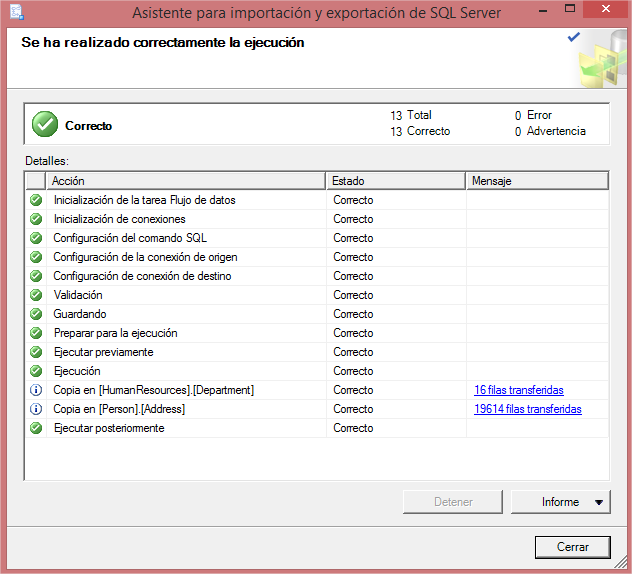
\includegraphics[width=18cm]{./Imagenes/imagen1}
		\end{center}
		\end{figure}

     	\item2. Conectandose con la base de datos AdventureWorks 
		\begin{figure}[H]
		\begin{center}
		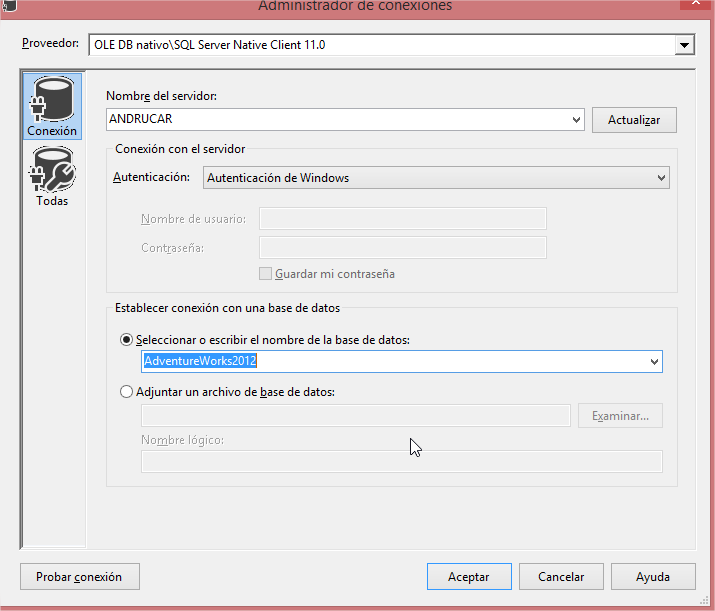
\includegraphics[width=18cm]{./Imagenes/imagen2}
		\end{center}
		\end{figure}
     

	\item3. Se configura el ejecutor de SQL
		\begin{figure}[H]
		\begin{center}
		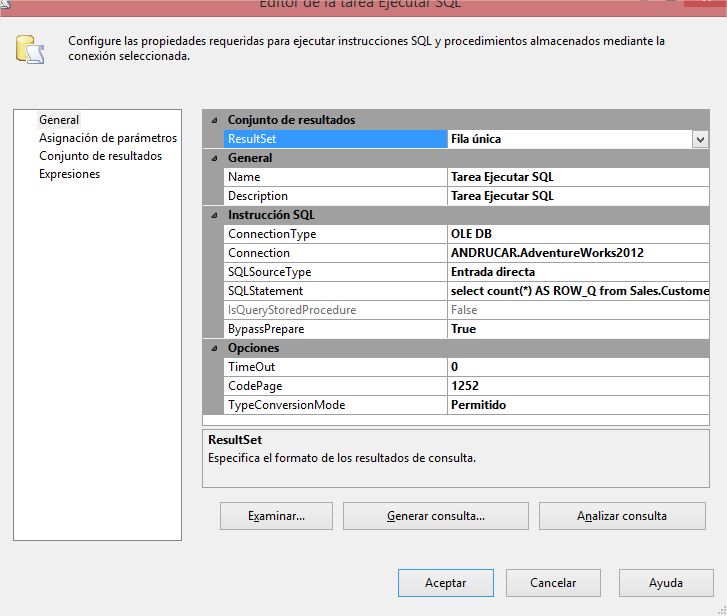
\includegraphics[width=18cm]{./Imagenes/imagen3}
		\end{center}
		\end{figure}
     
	\item 4. Resultado
		\begin{figure}[H]
		\begin{center}
		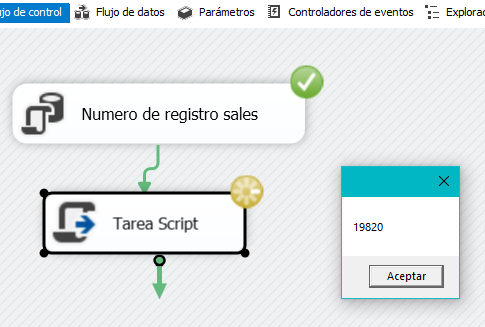
\includegraphics[width=18cm]{./Imagenes/imagen4}
		\end{center}
		\end{figure}
     
	\item 5. Conectadonse para cargar la siguiente base de datos AdventureWorks2017
		\begin{figure}[H]
		\begin{center}
		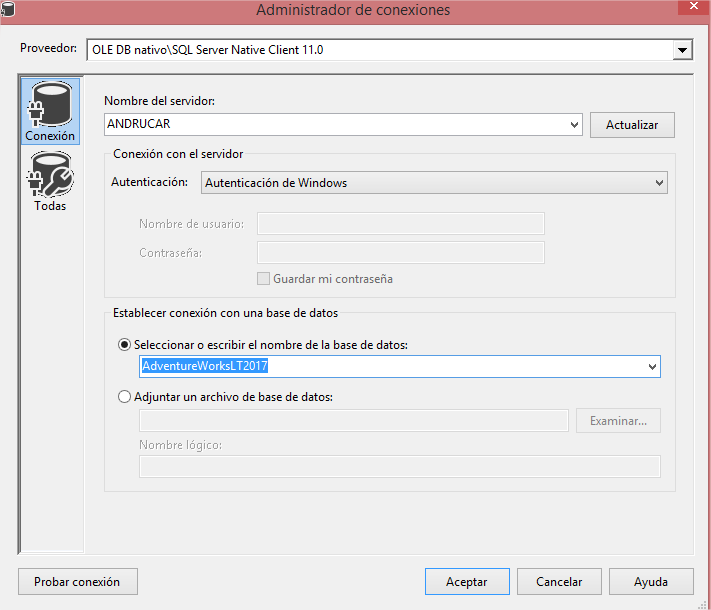
\includegraphics[width=18cm]{./Imagenes/imagen5}
		\end{center}
		\end{figure}
     
     
	\item 6. Datos de clientes en la tabla customer cargados correctamente
		\begin{figure}[H]
		\begin{center}
		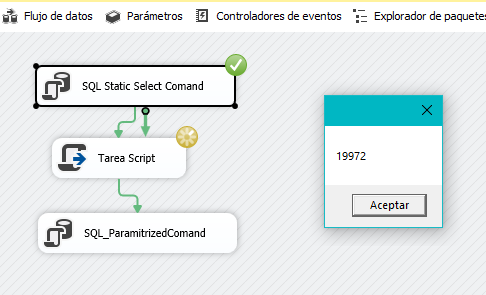
\includegraphics[width=18cm]{./Imagenes/imagen6}
		\end{center}
		\end{figure}
     



\end{itemize}
		